\chapter{Campionamento: cuti, piccoli campioni e biopsie}

Il campionamento delle biopsie e delle piccole resezioni viene trattato separatamente rispetto ai campioni chirurgici, poiché questi ultimi spesso non richiedono orientamento e non necessitano di un campionamento macroscopico mirato. In altre parole, viene effettuata una selezione casuale del materiale da inviare per l'analisi, mentre il resto del materiale viene conservato per eventuali ulteriori esami. Si noti che per le resezioni di grandi dimensioni o per le radicalizzazioni post-chirurgiche può essere necessaria la conservazione del campione.

Il campionamento di solito segue procedure standardizzate, con campionamento a "caso", ovvero campionando solo una parte del materiale senza una selezione accurata. La prima sezione di questo capitolo è dedicata alle biopsie cutanee.

\section{Biopsie Cutanee}

Le biopsie cutanee possono essere eseguite in qualsiasi ambulatorio e possono essere classificate in due categorie principali: biopsie incisionali e biopsie escissionali. Le biopsie incisionali prevedono il prelievo di solo una parte della lesione, mentre le biopsie escissionali mirano all'asportazione totale del tessuto ritenuto patologico.

Tra i tipi di campioni operatori che possono essere inviati al laboratorio vi sono:

\subsection{Biopsia Punch}
La biopsia punch consiste in un prelievo a carota di tessuto, che include l'epidermide e il derma. Se il punch è eseguito in profondità, può includere anche la quota di tessuto sottocutaneo. Viene utilizzato un cilindro metallico tagliente, appoggiato sulla cute, per estrarre una carota di tessuto. I punch sono disponibili in vari diametri e vengono frequentemente utilizzati per piccole lesioni o per malattie infiammatorie della pelle. A seconda delle dimensioni del punch, si può decidere se includere l'intero campione o suddividerlo per analizzare la lesione al centro del punch stesso. In caso di malattie infiammatorie, è spesso necessario congelare metà del campione per effettuare ulteriori analisi.

\subsection{Biopsia Shave}
La biopsia shave prevede l'abrasione della lesione cutanea, che può essere piatta o rilevata, mediante l'uso di una lama. Vengono rimosse solo le porzioni più superficiali del derma. È importante indicare il margine e il piano profondo per orientare il tecnico all'inclusione e per valutare la radicalità chirurgica.


\begin{figure}[p]
    \centering
    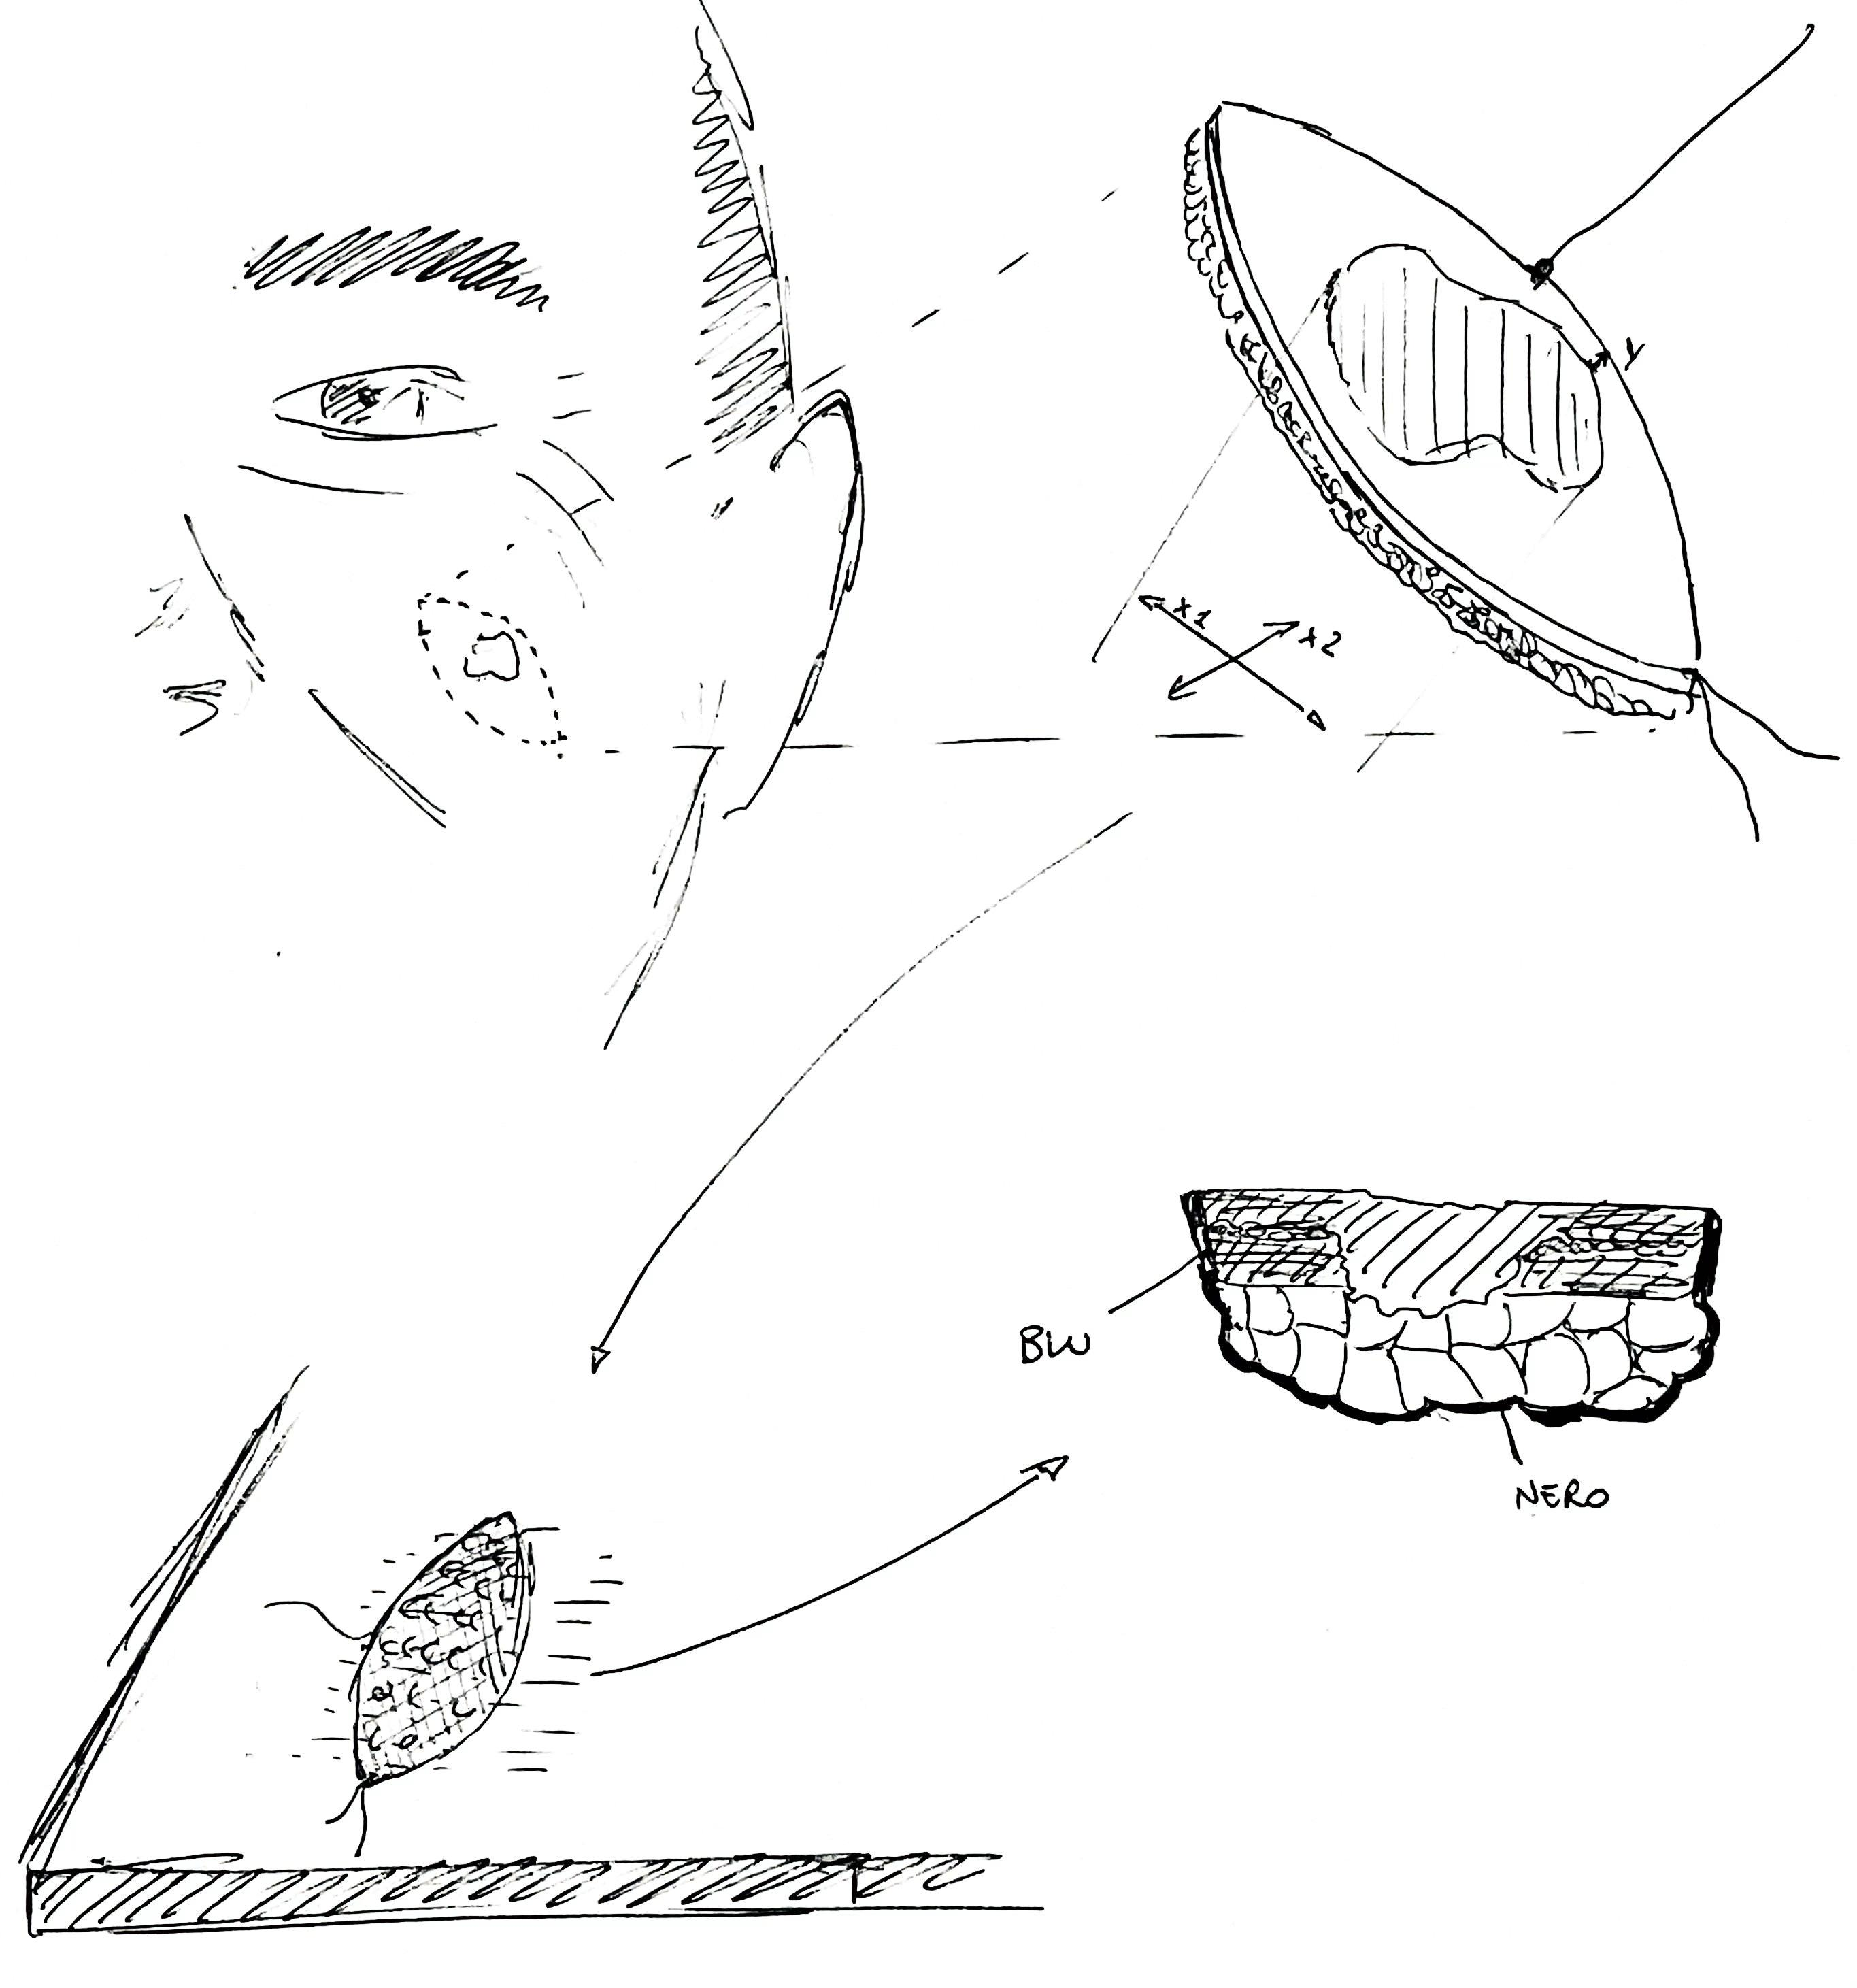
\includegraphics[width=0.75\textwidth]{campionamento_cute}
    \caption{Il campionamento delle losanghe cutanee.}
    \label{fig:campionamento_cute}
\end{figure}


\subsection{Losange Cutanee}
Le biopsie a forma di losanga prevedono un campione cutaneo con una forma romboidale, caratterizzato da due angoli acuti e due angoli arrotondati. Questa forma consente una migliore gestione chirurgica della ferita, con i due angoli acuti utilizzati come punto di partenza per la sutura. Le losange possono essere orientate, soprattutto in siti con margini ristretti, come sul volto, per facilitare l'asportazione di tessuto in caso di margine positivo.

\subsection{Descrizione Macroscopica}
Nella descrizione dei campioni cutanei è cruciale fornire dettagli macroscopici, per due motivi principali: primo, una diagnosi preliminare può essere fatta basandosi sull'aspetto macroscopico; secondo, la presenza di non concordanza tra la descrizione macroscopica e quella microscopica può suggerire ulteriori indagini. La descrizione delle neoformazioni cutanee deve includere dimensioni (in millimetri), caratteristiche morfologiche (rilevate, piatte, depressed), e dettagli sulla superficie (croste, escoriazioni, ulcere), oltre ai margini (netti o sfumati) e al colore, che è rilevante sia per lesioni melanocitarie che non melanocitarie.
